%--------------------------------------------------------------------------
% !TEX root = 5Blman.tex
% dc2.tex
% 2013.01.07 changed to 2col format
%--------------------------------------------------------------------------
\chapter {DC Circuits Part II}

\begin{multicols}{2}
%---------------------------------------------------------------------
\section {Purpose}  
The purpose of the first part of this laboratory exercise is to explore the internal resistance of an emf.  The purpose of the second part is to analyze a circuit that is not a simple combination of series and parallel connections.  You will measure currents in this circuit and compare the results to an analysis using Kirchhoff's rules.  The concepts of emf, terminal voltage, and internal resistance as well as Kirchhoff's rules are also explored in lecture, your text, and in homework questions and problems.  By exploring them in lab you will not only become more familiar with them, but also build your skills in the measurement and evaluation of voltage, current, and resistance.

%---------------------------------------------------------------------
\section {Preparation} Pay special attention in your text to the major features of terminal voltage and Kirchhoff's rules and to the associated problem-solving strategies for them.

\paragraph {Short quiz}  Be prepared to take a short quiz at the beginning of lab related to the concepts associated with this laboratory exercise.

%---------------------------------------------------------------------
\section {General Information}
\paragraph {Warning}  You are already aware that ammeters (meters used to measure current) are particularly vulnerable to damage.  If you are not certain that you have correctly connected your ammeter have your instructor check your connections before you close the switch(es) that apply voltage to the circuit.

%---------------------------------------------------------------------
\section {DC Circuits}

%\begin{figure}
%	\centering
%	\includegraphics[scale=0.6]{5bgraf/vimtr} %{5bgraf/fig_8}
%	\caption{Setup to measure internal resistance of a battery}
%	\label{f:vimtr}
%\end{figure}

\begin{center}
%	\includegraphics[scale=1]{5bgraf/vimtr} %{5bgraf/fig_8}
	\includegraphics[scale=0.6]{5bgraf/vimtr} %{5bgraf/fig_8}
	\mfcaption{Setup to measure internal resistance of a battery}
	\label{f:vimtr}
\end{center}

\subsection{Activity: Internal resistance of a battery}
\begin{enumerate}
	 \item Set up the circuit shown in \reffig{f:vimtr}.  Use a precision resistor for $R$ and estimate the current that will flow so that you can choose an appropriate scale for the ammeter.
	\item Measure and record the current and terminal voltage as accurately as possible: $V_T$ = the terminal voltage, $E$ = the $emf$, $I$ = the current, and $r$ = the internal resistance.
%	\item Measure and record the current and terminal voltage as accurately as possible. The terminal voltage is defined below with $V_T$ = the terminal voltage, $E$ = the $emf$, $I$ = the current, and $r$ = the internal resistance.

\begin{equation} \label{e:vterm}
	V_T  =  E -Ir 	%\quad \text{with E = emf voltage}	
\end{equation}
	\item Replace the precision resistor with one having a different resistance and repeat the measurements of current and terminal voltage.
	\item Calculate the internal resistance $r$ of the battery for each resistor. Measure the the emf of the battery with nothing connected to it, and measure $V_T$ for each resistor.  Are your values consistent?  If not, it may be that the internal resistance actually varies with load.
\begin{equation} \label{e:rintern}
	r  =  \dfrac{E - V_T}{I} = \dfrac{E - IR}{I}	%\quad \text{with E = emf voltage}	
\end{equation}

	\item Discuss these results and your observations regarding the internal resistance of your battery in your lab report.
\end{enumerate}

%\begin{figure}
%	\centering
%	\includegraphics[scale=0.7]{5bgraf/kvlr3}	 %{5bgraf/fig_9}
%	\caption{Multiloop circuit with 3 unknown currents}
%	\label{f:kvlr3}
%\end{figure}

%\begin{center}
%	\includegraphics[scale=0.6]{5bgraf/kvlr3}	 %{5bgraf/fig_9}
%	\mfcaption{Multiloop circuit with 3 unknown currents}
%	\label{f:kvlr3}
%\end{center}

\subsection{Activity: Kirchoff's rules}
%\begin{figure}
%	\centering
%	\includegraphics[scale=0.7]{5bgraf/kvlr3}	 %{5bgraf/fig_9}
%	\caption{Multiloop circuit with 3 unknown currents}
%	\label{f:kvlr3}
%\end{figure}

\begin{center}
	\includegraphics[scale=0.6]{5bgraf/kvlr3}	 %{5bgraf/fig_9}
	\mfcaption{Multiloop circuit with 3 unknown currents}
	\label{f:kvlr3}
\end{center}

\begin{enumerate}
	 \item Measure the emfs of both of your batteries.  Assuming the voltmeter has high resistance, the emf, $E$ is the voltage you measure with the battery alone connected to the voltmeter.
	\item Assemble the circuit shown in \reffig{f:kvlr3}.
	See \reffig{f:circboard} for a pictorial representation of the circuit.
	\item Measure the terminal voltages of your batteries with both tap keys held down.
	\item Using the block diagram of \reffig{f:circboard} on page \pageref{f:circboard} as a guide, measure the currents $I_1$, $I_2$, and $I_3$, --- remove the appropriate wire, insert the ammeter, then measure the current.
	See \reffig{f:fig10b} for a pictorial representation of the circuit.
%	\item Measure the terminal voltages of your batteries with both tap keys held down.
%	\item Using the block diagram of \reffig{f:fig10b} on page \pageref{f:fig10b} as a guide, measure the currents $I_1$, $I_2$, and $I_3$, --- remove the appropriate wire, insert the ammeter, then measure the current.

	\item Apply Kirchhoff's junction rule to junction $A$ and Kirchhoff's loop rule to the top and bottom loop.  Enter the values of the currents, resistances, and voltages for this circuit into each equation.  Are the rules verified by your values? Discuss your results.
	\item Solve the three equations obtained from the application of Kirchhoff's rules for the currents $I_1$, $I_2$, and $I_3$, treating them as unknowns. (Your instructor can provide some guidance in how to solve three equations for three unknowns.)
	\item Then calculate the currents using the known values of the resistances and voltages.  Compare the calculated values of the currents to the measured values and discuss how well they agree. 
\end{enumerate}

%\begin{figure} \centering
% \subfloat[circuit board]
%   {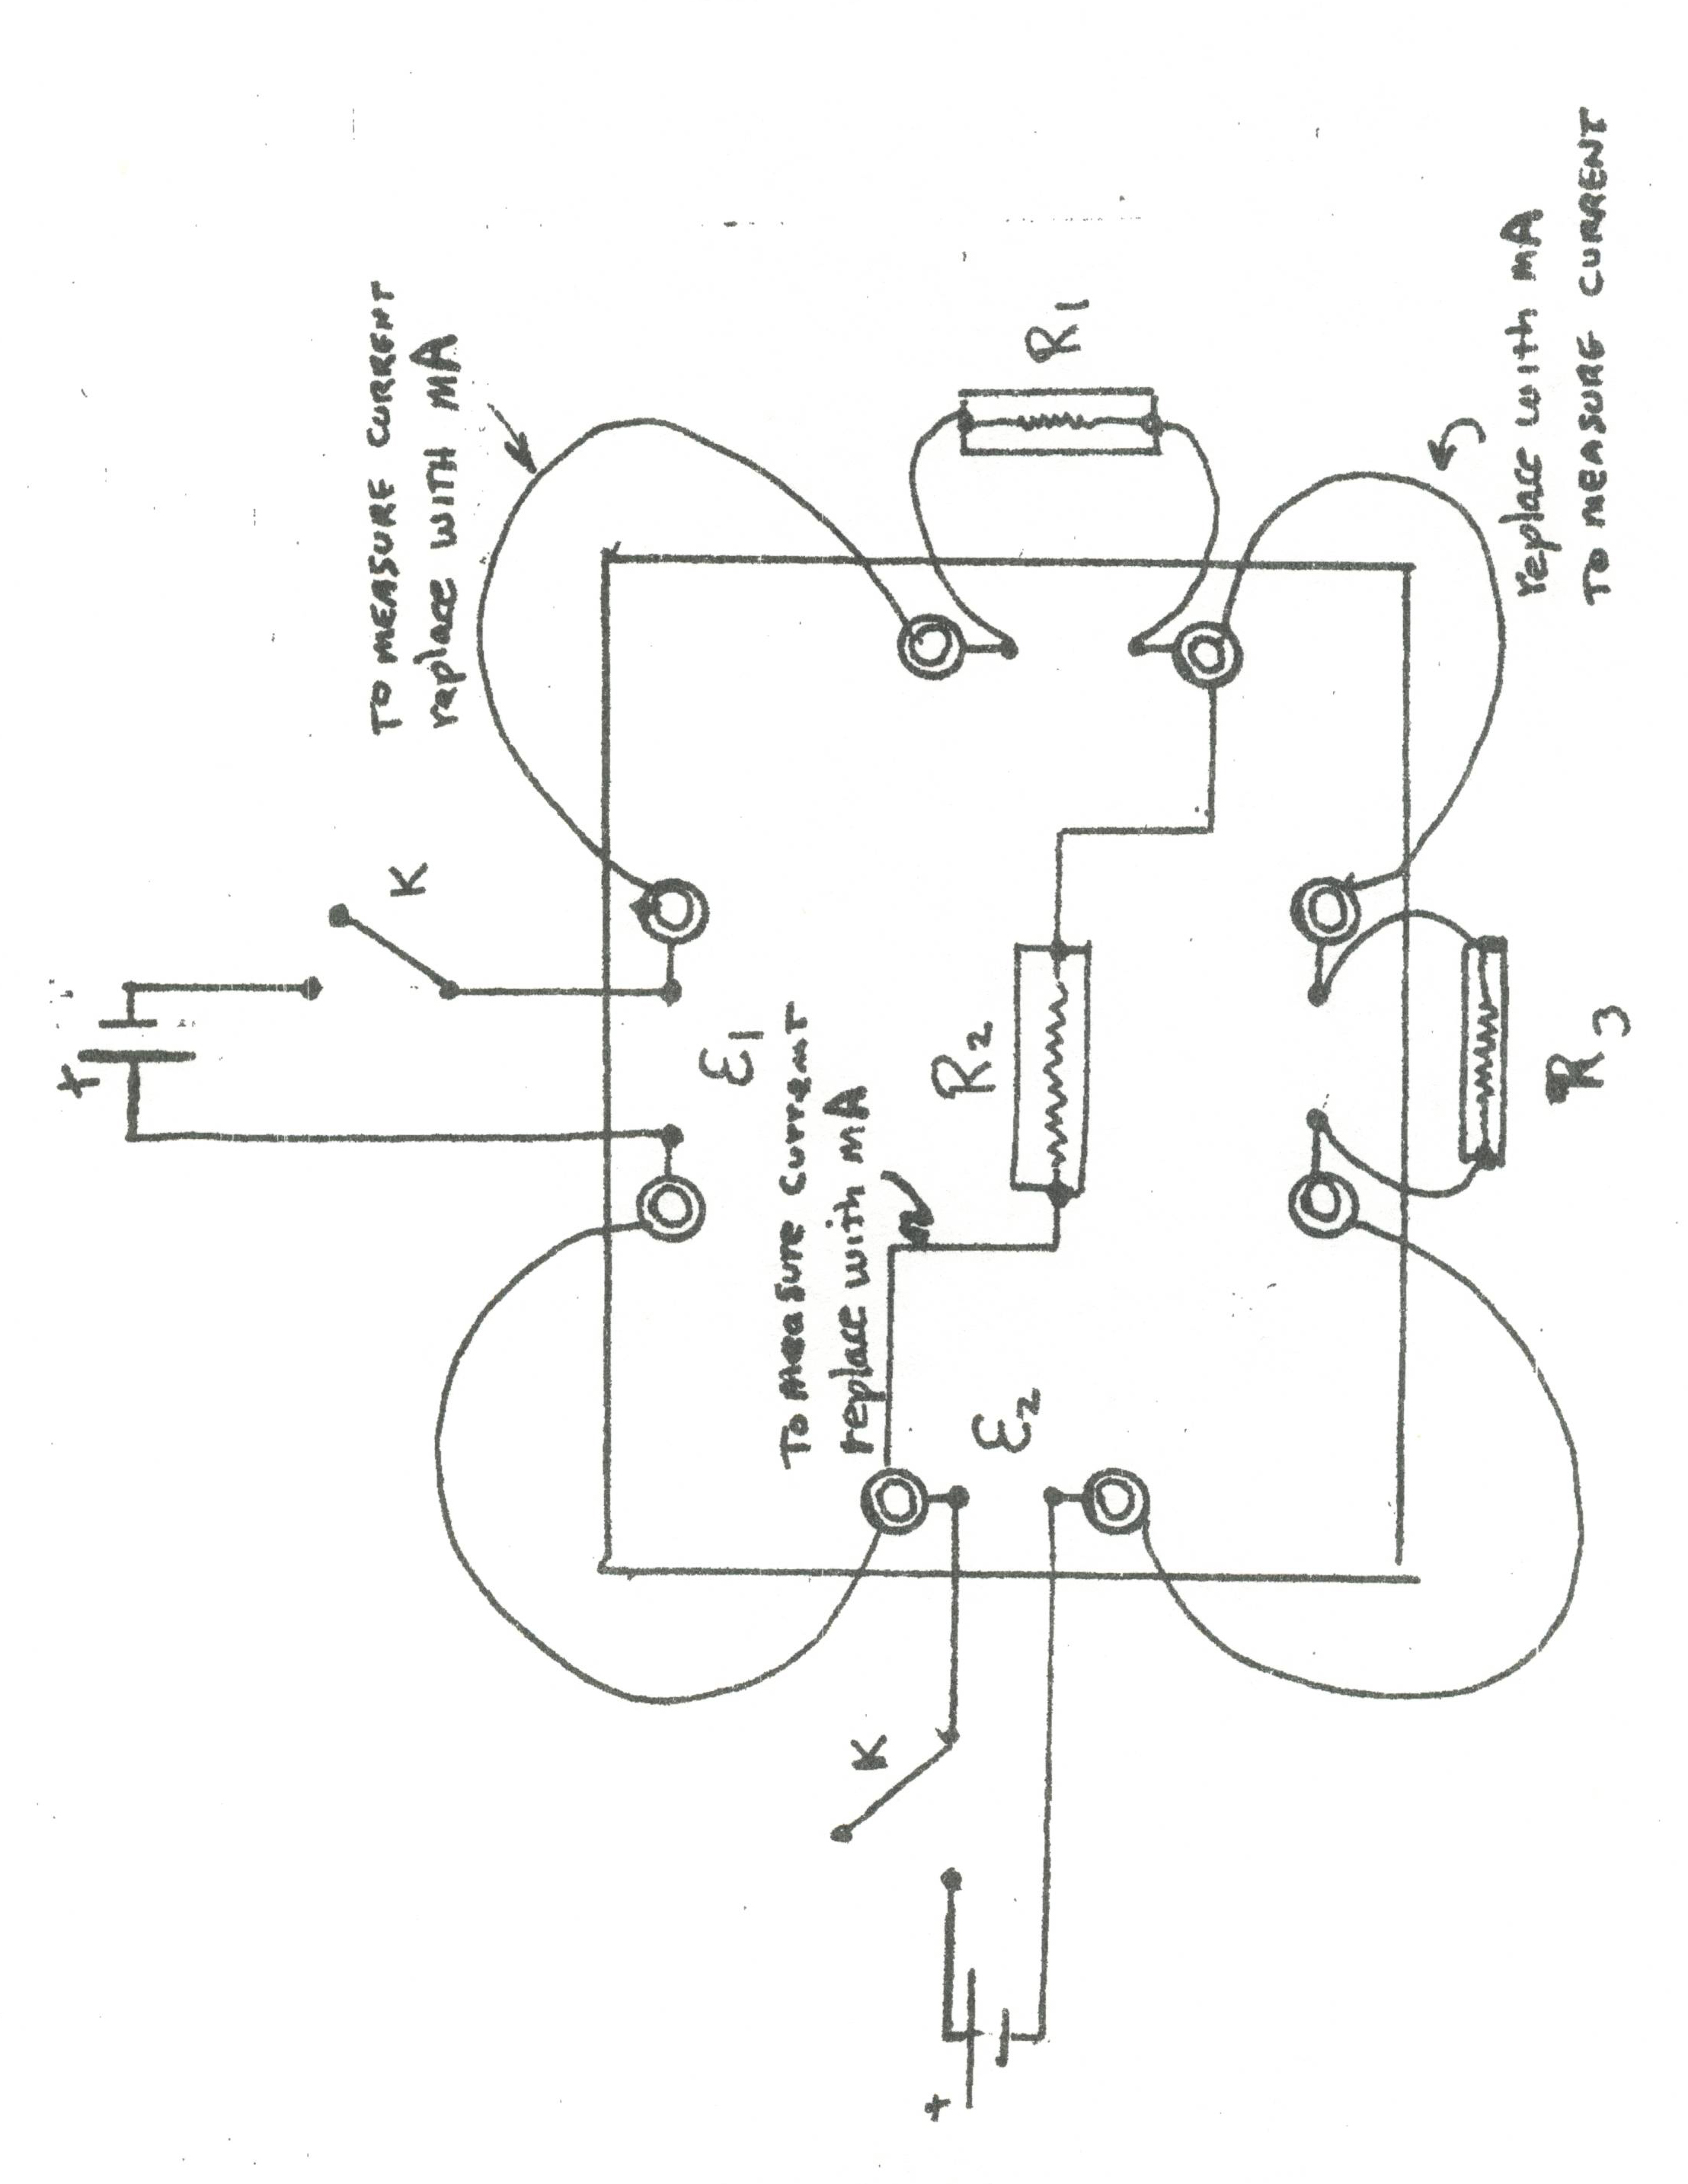
\includegraphics[scale=0.9]{5bgraf/fig_10b}\label{f:fig10b}}
%
% \subfloat[multimeter]
%   {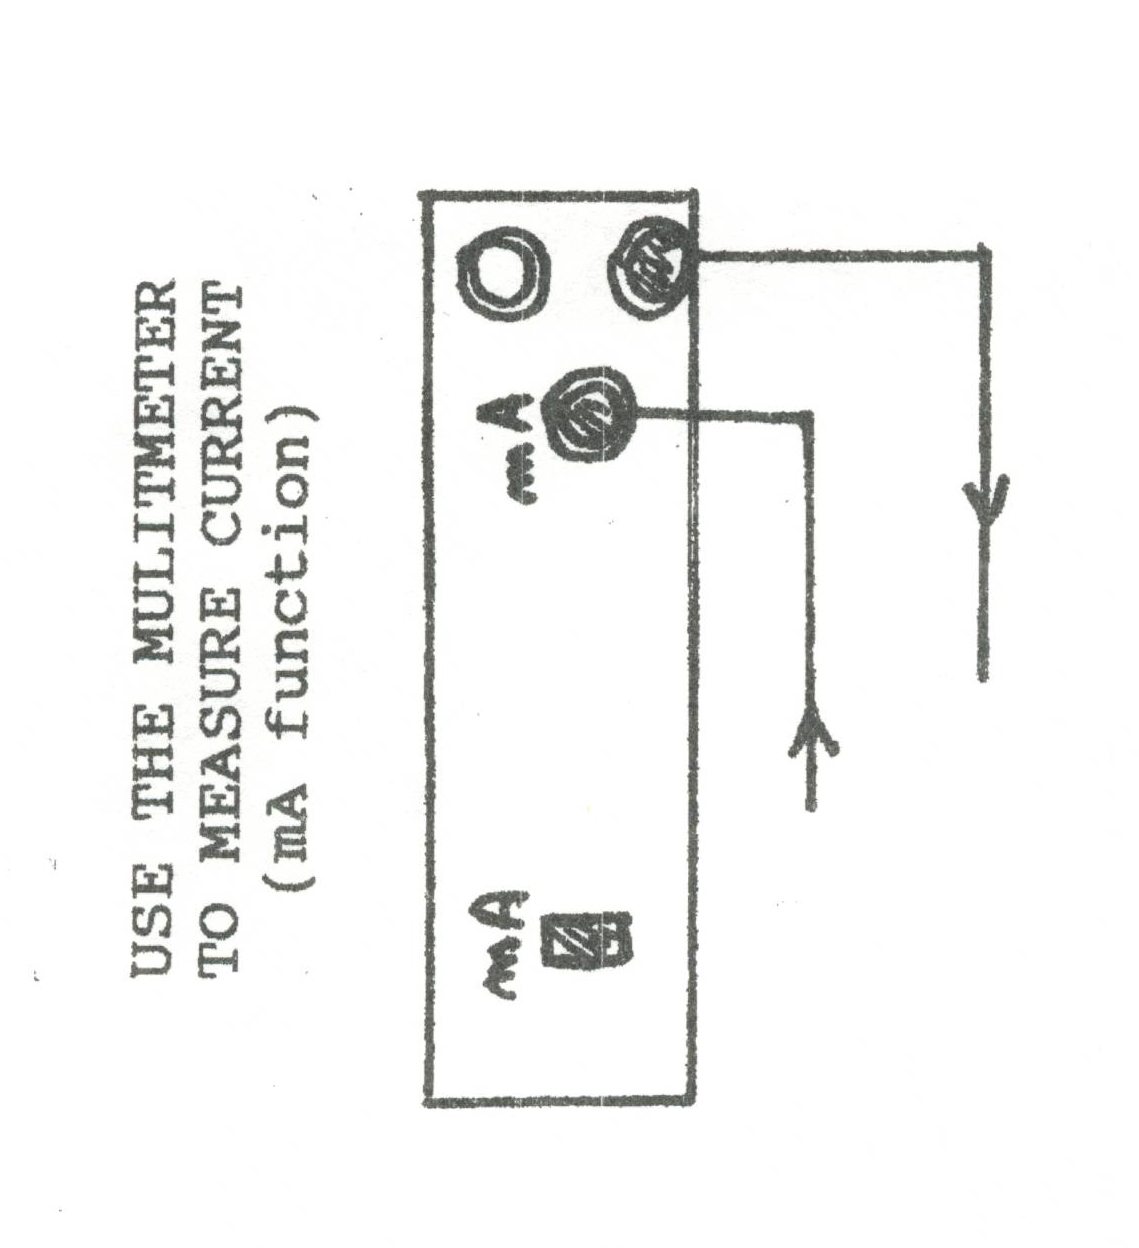
\includegraphics[scale=0.4]{5bgraf/fig_10a}\label{f:fig10a}}
% \caption{Circuit board arrangement for Kirchoff's rules}\label{f:circboard}
%\end{figure}
\end{multicols}

\begin{center}
   {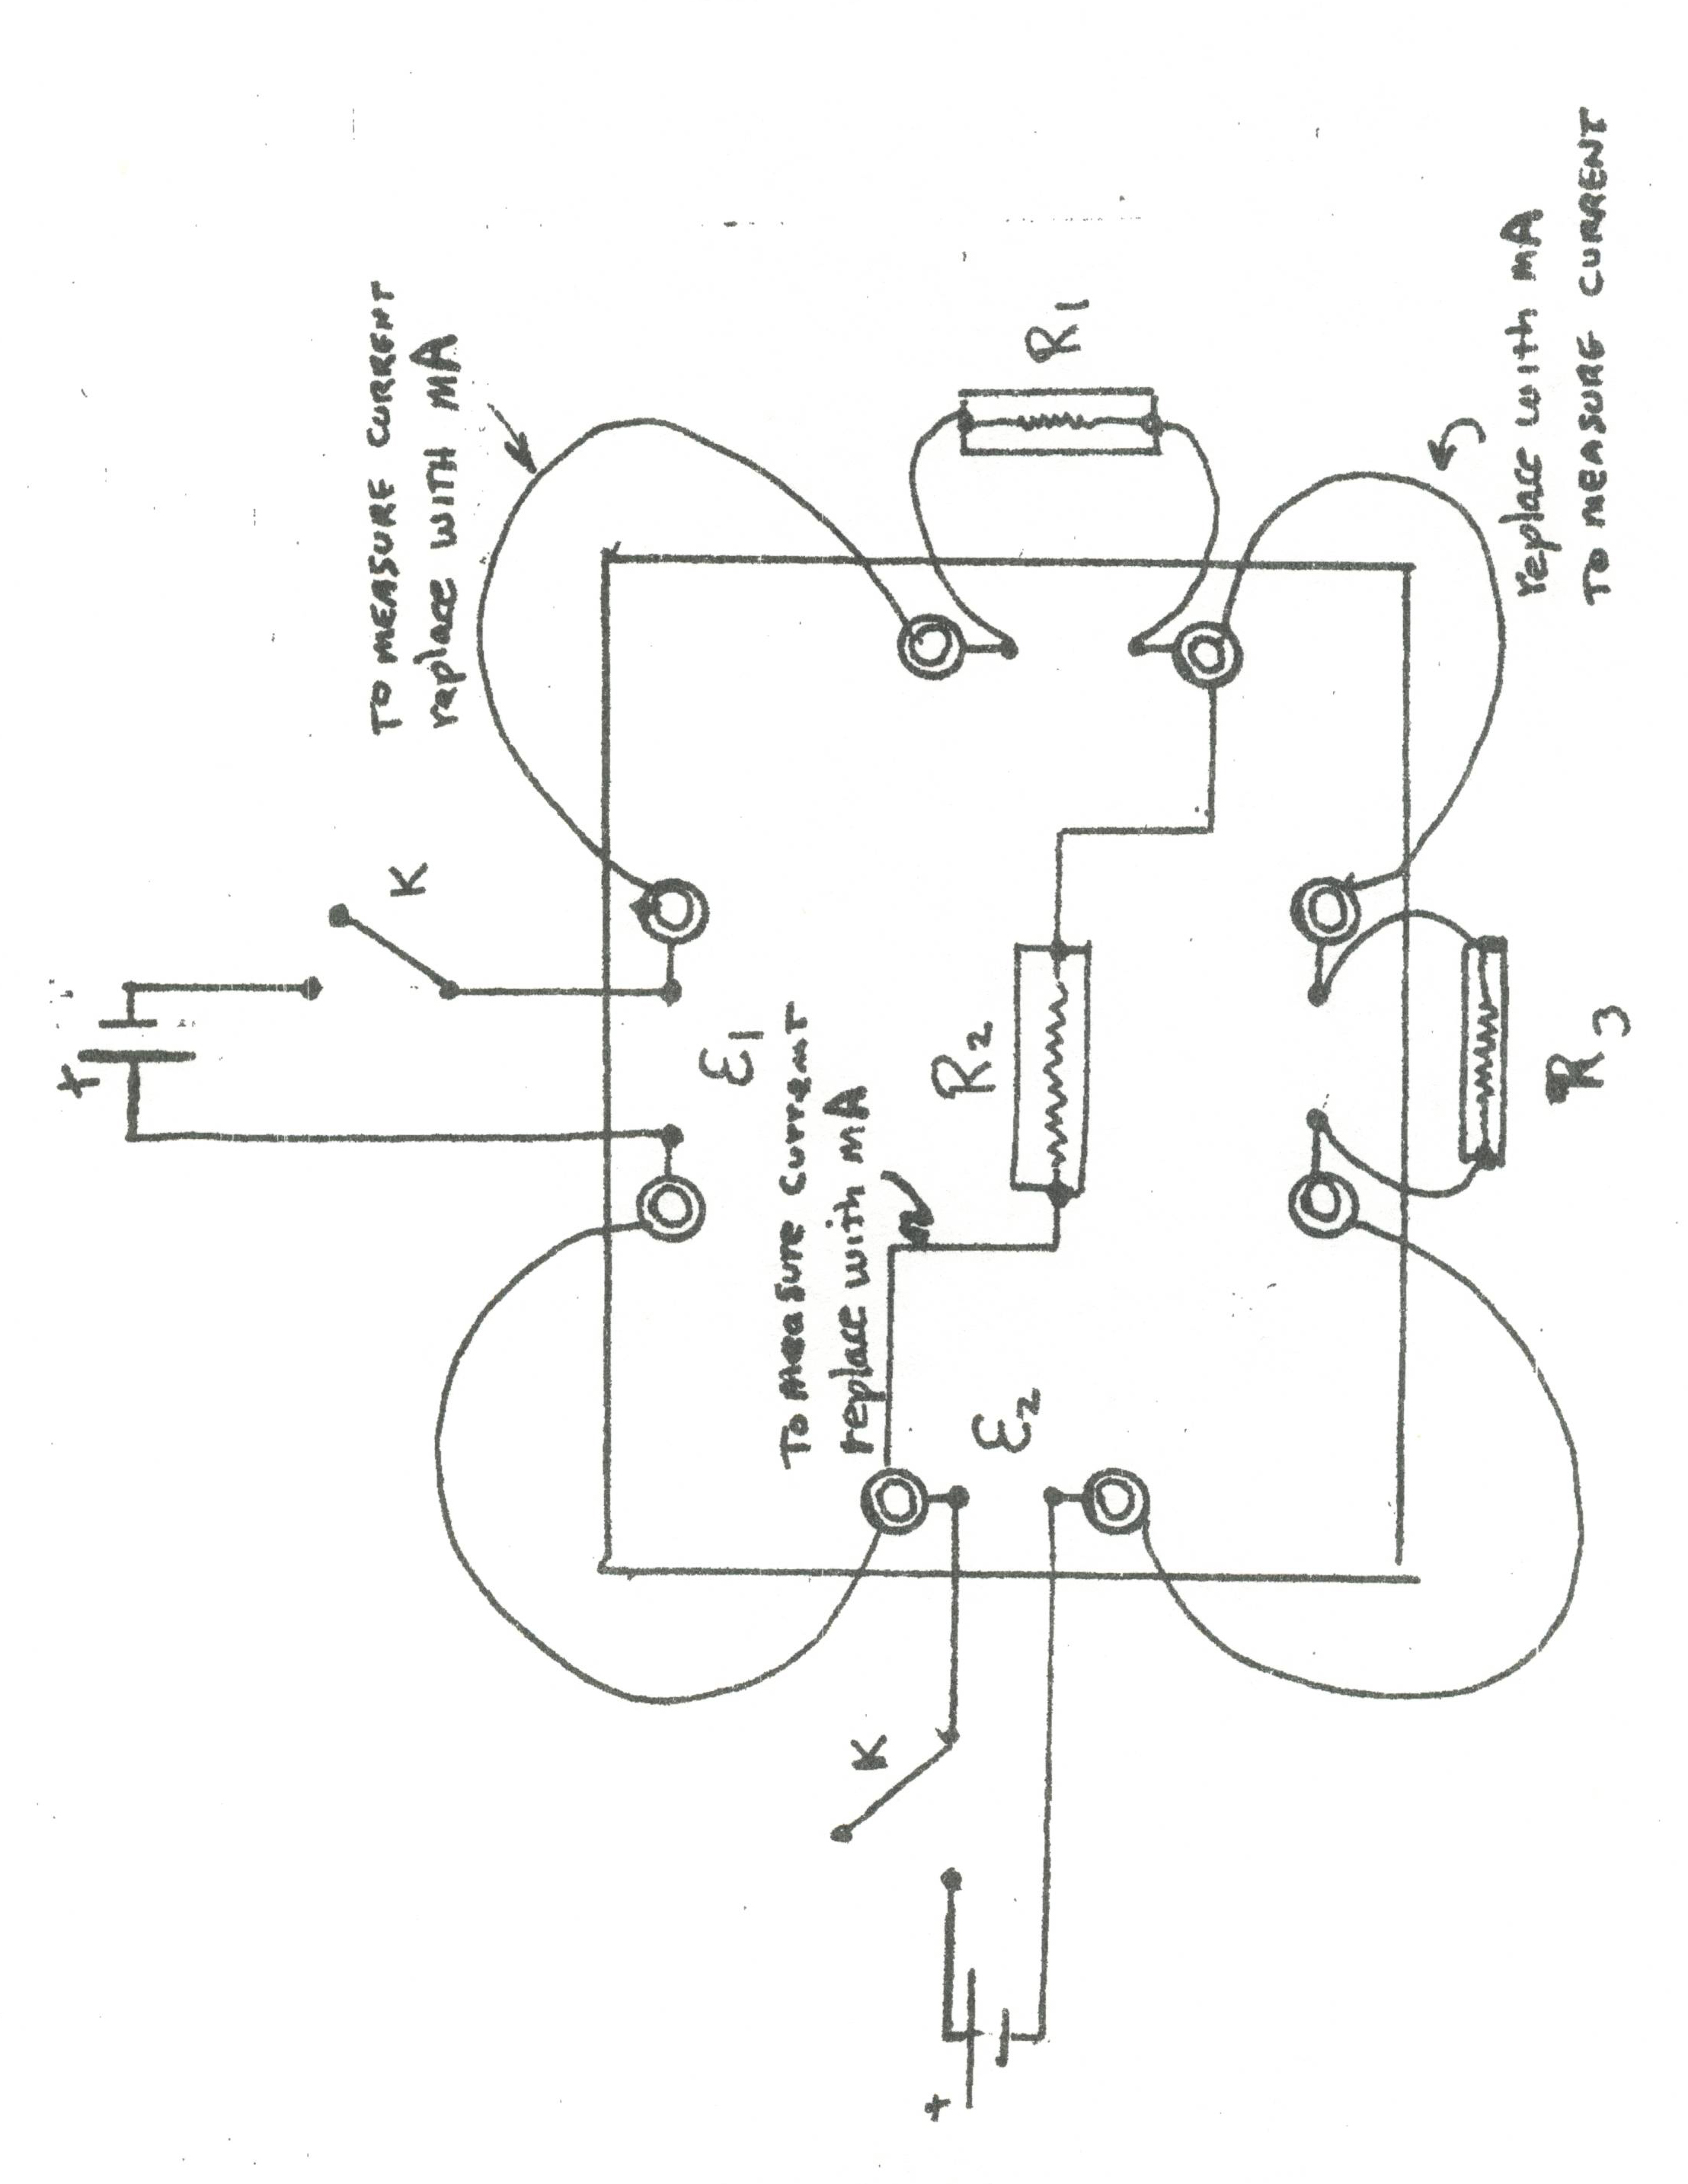
\includegraphics[scale=0.9]{5bgraf/fig_10b}\label{f:fig10b}}
   {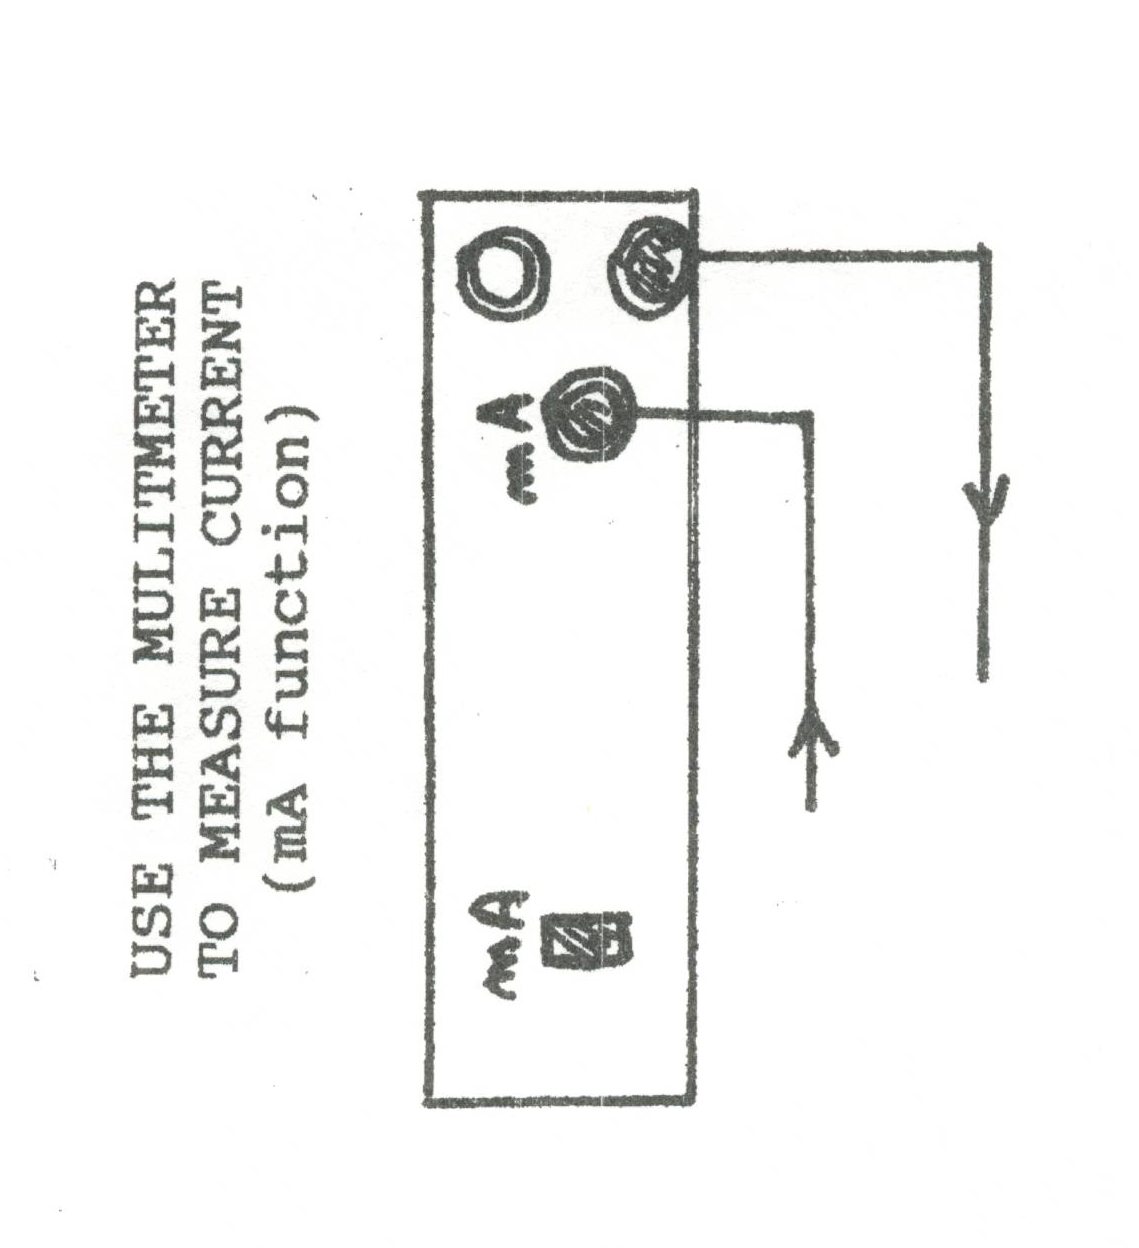
\includegraphics[scale=0.4]{5bgraf/fig_10a}\label{f:fig10a}}
	\mfcaption{Circuit board arrangement for Kirchoff's rules}\label{f:circboard}
\end{center}


\paragraph {Conclusions:}  What general conclusions can you make concerning the internal resistance of batteries and the application of Kirchhoff's rules?

%--begin comment---------------------------------------------------------
\begin{comment}
\begin{enumerate}
	\item Determining the Internal Resistance of a Battery
	\begin{enumerate}
		\item Set up the following circuit.  Use a precision resistor for $R$ and estimate the current that will flow so that you can choose an appropriate scale for the ammeter.

\begin{figure}
	\centering
	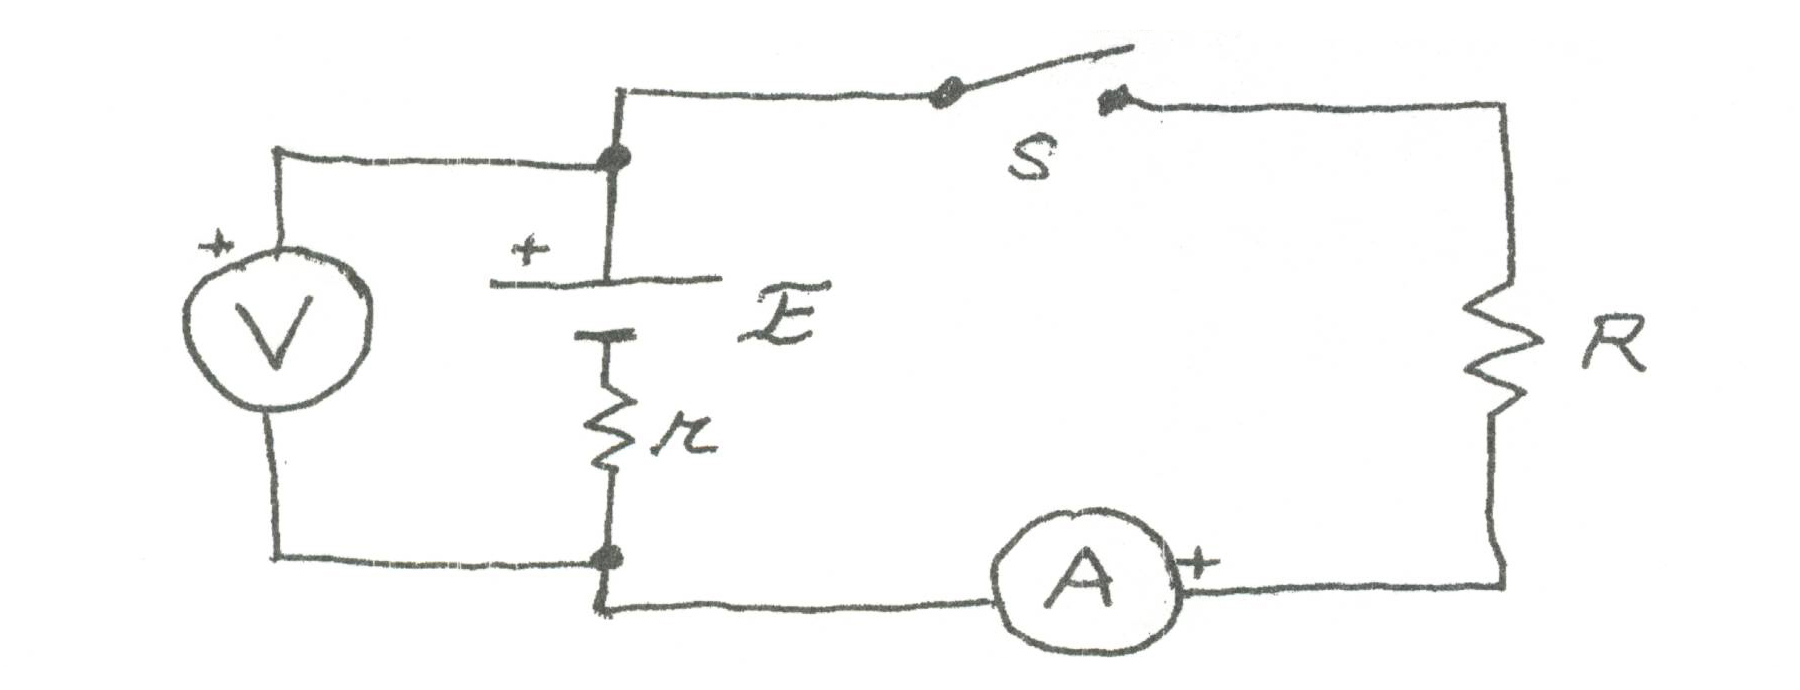
\includegraphics[scale=0.8]{5bgraf/fig_8}
	\caption{Setup to measure internal resistance of a battery}
	\label{f:fig8}
\end{figure}

		\item Measure and record the current and terminal voltage as accurately as possible.
		\item Replace the precision resistor with one having a different resistance and repeat the measurements of current and terminal voltage.
		\item Calculate the internal resistance $r$ of the battery for each measurement taking the emf to be $E = 1.54 V$.  Are your values consistent?  If not, it may be that the internal resistance actually varies with load.  Discuss these results and your observations regarding the internal resistance of your battery in your lab report.
	\end{enumerate}
	\item Kirchhoff's rules
	
	\begin{enumerate}
		\item Measure the emfs of both of your batteries.  Assuming the voltmeter has high resistance, the emf, $E$ is the voltage you measure with the battery alone connected to the voltmeter.
		\item Assemble the circuit shown in fig. \ref{f:fig_9}.  (See fig. \ref{f:fig10b} for a pictorial representation of the circuit.)

\begin{figure}
	\centering
	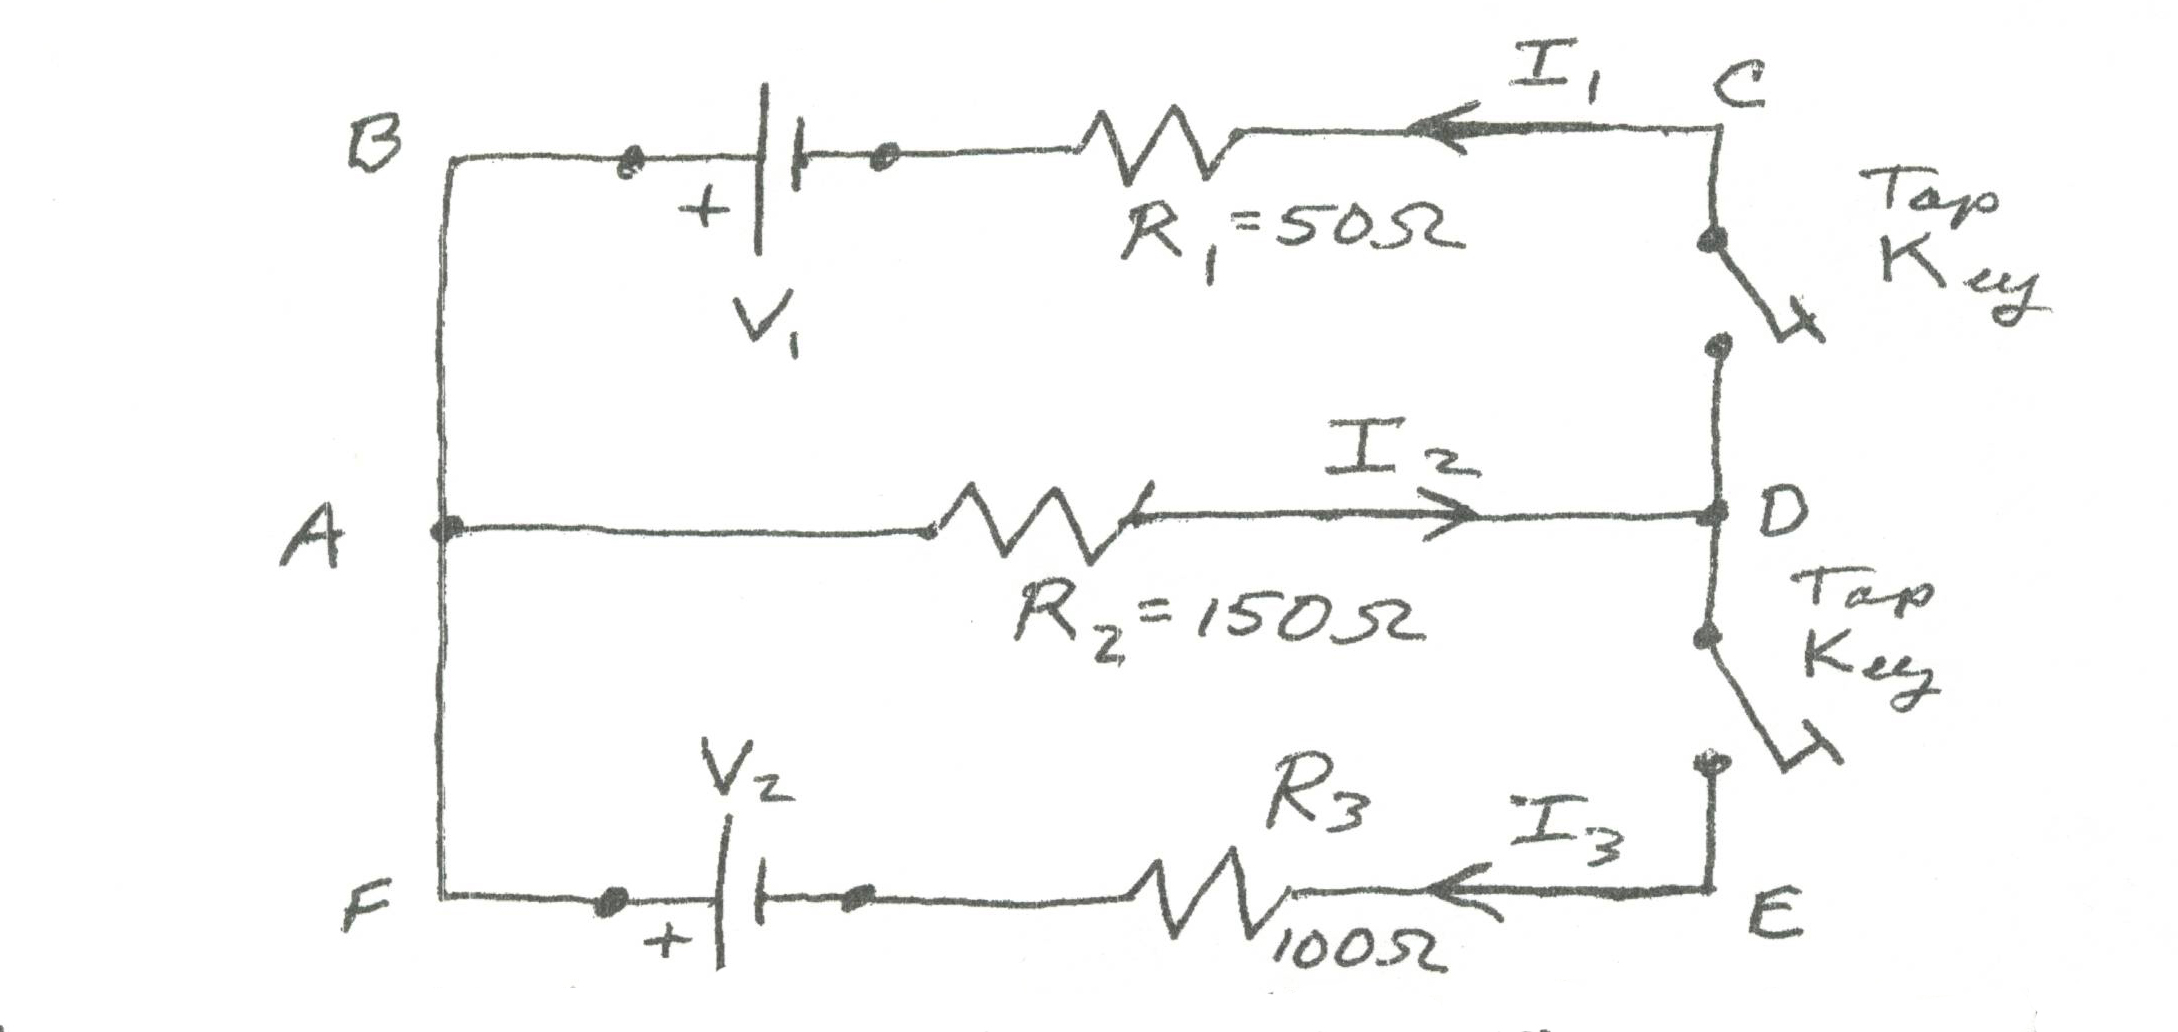
\includegraphics[scale=0.8]{5bgraf/fig_9}
	\caption{Multiloop circuit with 3 unknown currents}
	\label{f:fig9}
\end{figure}

		\item Measure the terminal voltages of your batteries with both tap keys held down.
		\item Using the diagram on the next page as a guide, measure the currents $I_1$, $I_2$, and $I_3$, by removing the appropriate wire and running the current that would flow through that wire through the ammeter.
		\item Apply Kirchhoff's junction rule to junction $A$ and Kirchhoff's loop rule to the top and bottom loop.  Enter the values of the currents, resistances, and voltages for this circuit into each equation.  Are the rules verified by your values? Discuss your results.
		\item Solve the three equations obtained from the application of Kirchhoff's rules for the currents $I_1$, $I_2$, and $I_3$, treating them as unknowns.  (Your instructor will provide some guidance in how to solve three equations for three unknowns.)  Then calculate the currents using the known values of the resistances and voltages.  Compare the calculated values of the currents to the measured values and discuss how well they agree.
	\end{enumerate}
\end{enumerate}
\end{comment}
%--end comment----------------------------------------------------------


%\begin{figure}
%	\centering
%	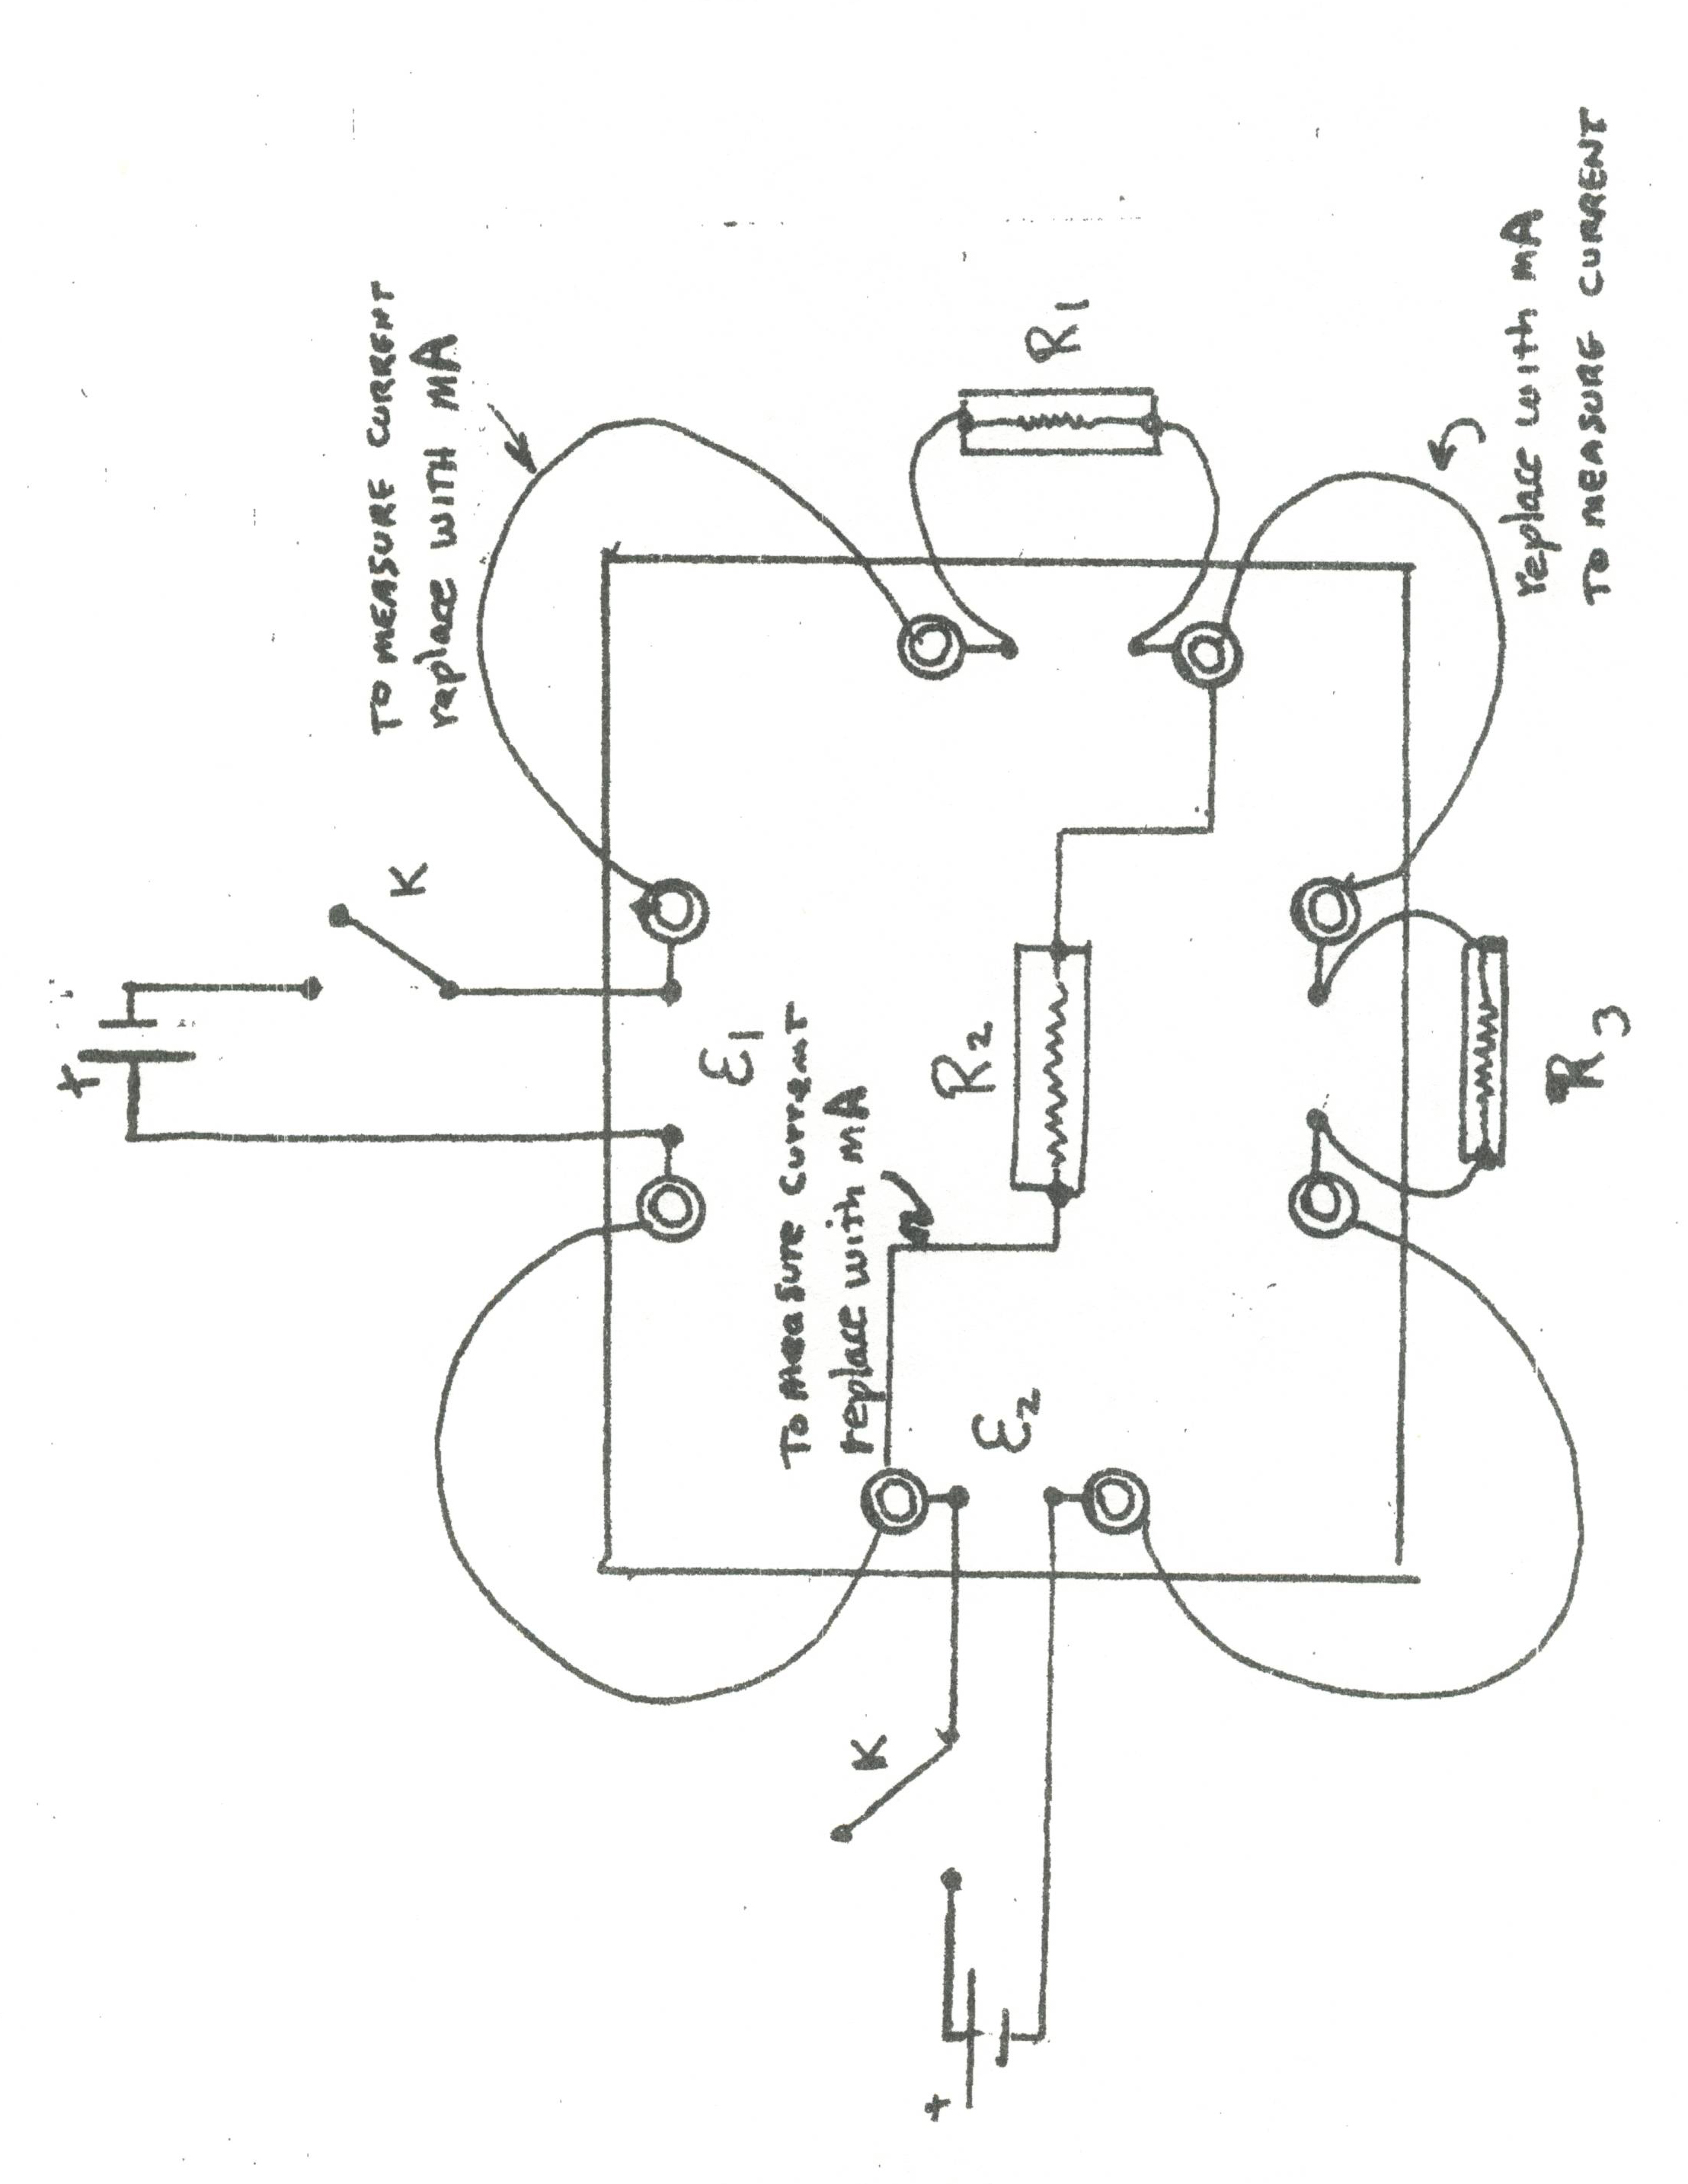
\includegraphics[scale=0.8]{5bgraf/fig_10b}
%	\caption{Circuit board arrangement for Kirchoff's rules}
%	\label{f:fig10b}
%\end{figure}

%\begin{figure}
%	\centering
%	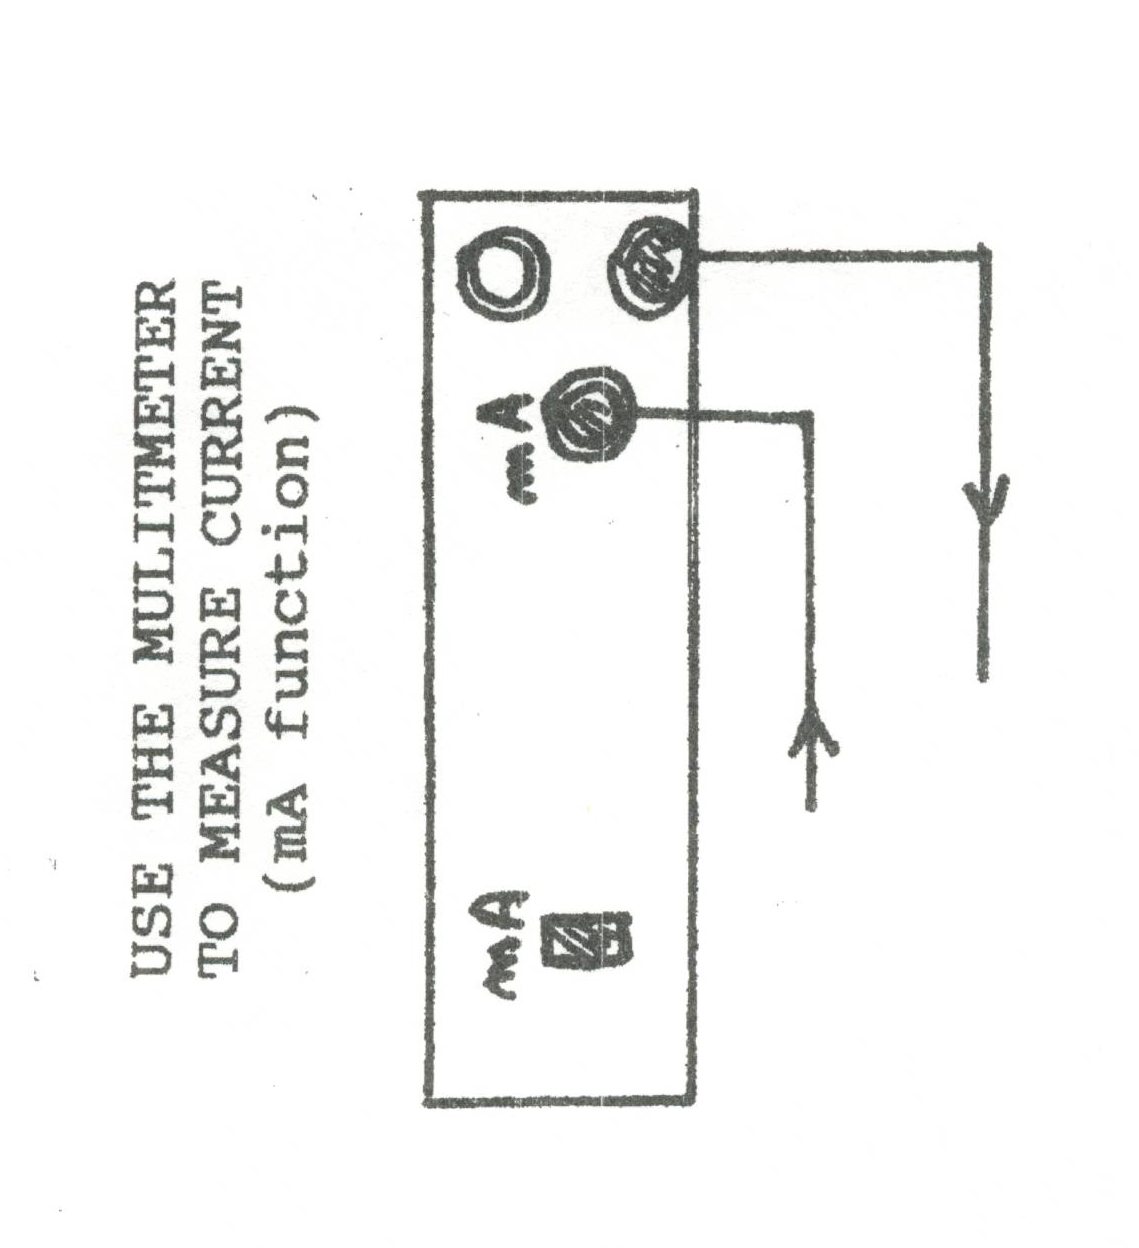
\includegraphics[scale=0.4]{5bgraf/fig_10a}
%	\caption{Multimeter for current measurement}
%	\label{f:fig10a}
%\end{figure}

%--------------------------------------------------------------------------
\endinput
%--------------------------------------------------------------------------
